\documentclass[conference]{IEEEtran}
% The preceding line is only needed to identify funding in the first footnote. If that is unneeded, please comment it out.
\usepackage{amsmath,amssymb,amsfonts}
\usepackage{algorithm2e}
\RestyleAlgo{ruled}
\usepackage{graphicx}
\usepackage{textcomp}
\usepackage{xcolor}
\usepackage{subcaption}
\usepackage{booktabs}
\usepackage{tabularx}
\usepackage{multirow}
\usepackage[style=numeric,sorting=none]{biblatex}
\addbibresource{reference.bib}
\def\BibTeX{{\rm B\kern-.05em{\sc i\kern-.025em b}\kern-.08em
    T\kern-.1667em\lower.7ex\hbox{E}\kern-.125emX}}
\begin{document}

\title{Solving the Adult Census Income Prediction Problem with Principal Component Analysis and Light Gradient Boosting Machine}

\author{
    \IEEEauthorblockN{Mengxuan Wu}
    \IEEEauthorblockA{
        \textit{Department of Computer Science and Engineering} \\
        \textit{Southern University of Science and Technology} \\
        12212006@mail.sustech.edu.cn
    }
}

\maketitle

\begin{abstract}
    The Adult Census Income Prediction Problem is a binary classification problem that aims to predict whether a person earns more than 50,000 dollars a year based on the census data.
    In this report, we present a solution to this problem by applying Principal Component Analysis (PCA) to reduce the dimensionality of the data and then training multiple classifiers with different algorithms.
    We then evaluate the performance of these classifiers by comparing their F1 scores.
    Our results show that the Light Gradient Boosting Machine (LGBM) classifier achieves the best performance with an F1 score of 0.6357.
\end{abstract}

\section{Introduction}

The Adult Census Income Prediction Problem is a binary classification problem that aims to predict whether a person earns more than 50,000 dollars a year based on the census data.
The dataset contains 14 features, including age, workclass, education, marital status, occupation, etc.
The target variable is the income level, which is divided into two classes: $>50$K and $<=50$K.

In this report, we present a solution to this problem by applying Principal Component Analysis (PCA) to reduce the dimensionality of the data and then training multiple classifiers with different algorithms.
We then evaluate the performance of these classifiers by comparing their F1 scores.

\section{Related Work}

\subsection{Principal Component Analysis}

Generally, real-world data may contain numerous features.
The curse of dimensionality, which refers phenomena that arise when analyzing and organizing data in high-dimensional spaces but do not occur in low-dimensional settings, can lead to overfitting and poor generalization.
This is because space grows exponentially with the number of dimensions, and the data points become sparse.
Therefore, it is often required to reduce the dimensionality of the data to improve the performance of machine learning algorithms, so-called \textbf{dimensionality reduction}.

Principal Component Analysis (PCA) is a popular technique for dimensionality reduction.
It is a linear transformation technique that projects the data onto a lower-dimensional space while preserving as much variance as possible.

For example, we use PCA to reduce the dimensionality of the ``Wine'' dataset from 13 features to 2 features.
Then, we apply random forest to classify the data.
Even though the dimensionality is greatly reduced, the classification accuracy only deceases by less than 2\% (from 100\% to 98.15\%).
So is the F1 score (from 1 to 0.9814).

\begin{figure}[!ht]
    \centering
    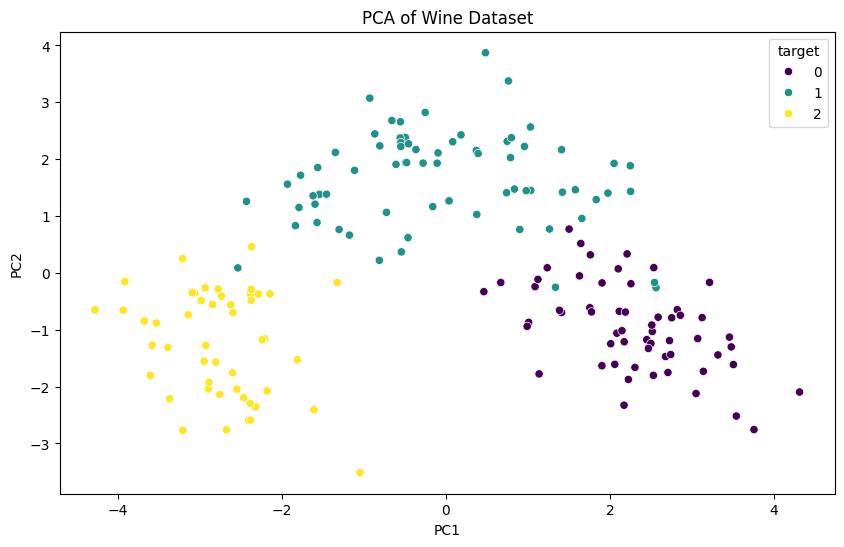
\includegraphics[width=\linewidth]{figure/Wine PCA.png}
    \caption{Scatter plot of the ``Wine'' dataset after PCA}
    \label{fig:wine_pca}
\end{figure}

\begin{figure}[!ht]
    \centering
    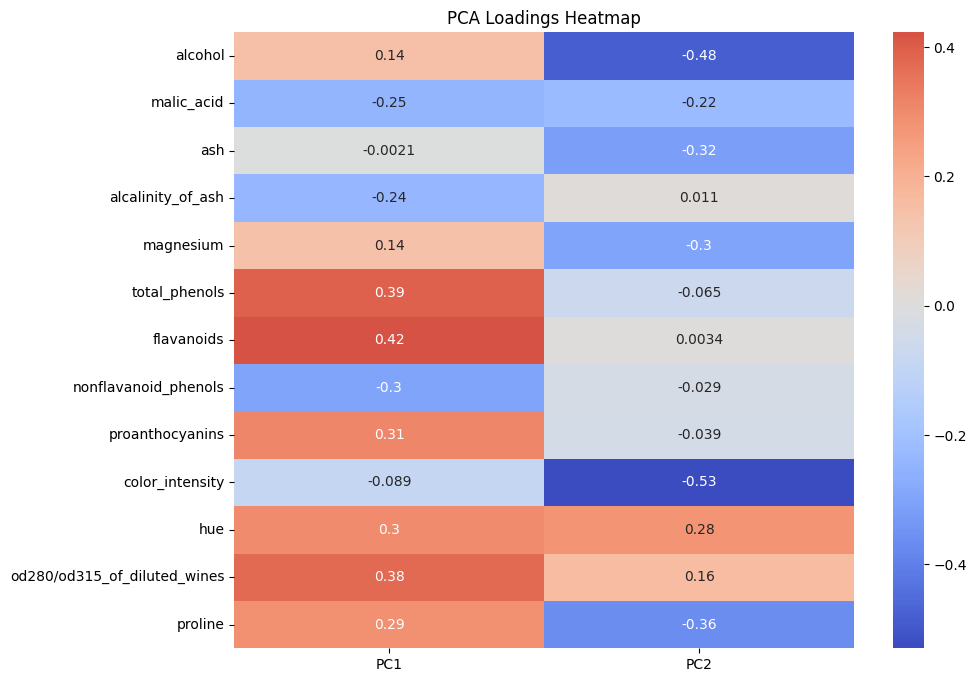
\includegraphics[width=\linewidth]{figure/Wine PCA Heatmap.png}
    \caption{Component relationship heatmap}
    \label{fig:wine_pca_heatmap}
\end{figure}

As shown in Figure \ref{fig:wine_pca}, the data points after PCA are well separated between different classes, which indicates that PCA is effective in reducing the dimensionality of the data while preserving the variance.

Also, it is worth noting that after PCA, the new features (components) are not the same as the original features.
Instead, it is a linear combination of the original features.
The relationship between the original features and the components can be visualized in the component relationship heatmap, as shown in Figure \ref{fig:wine_pca_heatmap}.

\subsection{Light Gradient Boosting Machine}

Light Gradient Boosting Machine (LGBM) \cite{zhang2017gpuacceleration} is a popular gradient boosting framework.
Its key technique, boosting, is an ensemble learning method that combines multiple weak learners to create a strong learner.
In each iteration, the model learns from the mistakes made by the previous models and updates the weights of the data points to focus on the misclassified points.
This process is repeated until the model converges.
In LGBM, the weak learners are decision trees.

Boosting is a powerful technique.
Among all the classifiers we have tested, boosting classifiers obtain 3 of the top 5 F1 scores.

\subsection{F1 Score}

The F1 score is the harmonic mean of precision and recall.
It is a good metric for imbalanced datasets because it takes both false positives and false negatives into account.
The F1 score is calculated as follows:
\begin{equation}
    \text{F1 Score} = 2 \times \frac{precision \times recall}{precision + recall}
\end{equation}
where precision and recall are defined as follows:
\begin{equation}
    \text{Precision} = \frac{TP}{TP + FP}
\end{equation}
\begin{equation}
    \text{Recall} = \frac{TP}{TP + FN}
\end{equation}

The superiority of the F1 score can be demonstrated by the following example.
Suppose we have a binary classification problem with 100 data points, where 95 data points belong to class 0 and 5 data points belong to class 1.
For a dummy classifier that always predicts class 0, the accuracy is 95\%.
However, the F1 score is 0 because the classifier fails to predict any data point in class 1.
This example shows that the F1 score is a better metric for imbalanced datasets than accuracy.

\section{Methodology}

\subsection{Data Preprocessing}

\subsubsection{Missing Values}

The dataset contains missing values, which are represented by a question mark.
For numerical features, we replace the missing values with the mean of the corresponding feature.
For categorical features, we replace the missing values with the mode of the corresponding feature (the most frequent value).

\subsubsection{Ordinal Encoding}

The dataset contains categorical features.
However, most machine learning algorithms require numerical input.
Therefore, we use ordinal encoding to convert the categorical features into numerical features.
In ordinal encoding, each unique category is assigned an integer value.
For example, the feature ``workclass'' has 9 unique categories, which are encoded as integers from 0 to 8.

\subsubsection{Normalization}

We use z-score normalization to normalize the numerical features.
For each numerical feature, we calculate the mean and standard deviation of the feature.
Then, we subtract the mean from each data point and divide by the standard deviation.

\subsection{Principal Component Analysis}

As mentioned earlier, PCA is a linear transformation technique that projects the data onto a lower-dimensional space while preserving as much variance as possible.
After the preprocessing steps mentioned above, we apply PCA to reduce the dimensionality of the data.
As shown in Figure \ref{fig:pca_explained_variance}, the explained variance ratio of the components decreases as the number of components increases.
We choose the number of components such that the explained variance ratio is greater than 0.95, which left the first 13 components.

\begin{figure}[!ht]
    \centering
    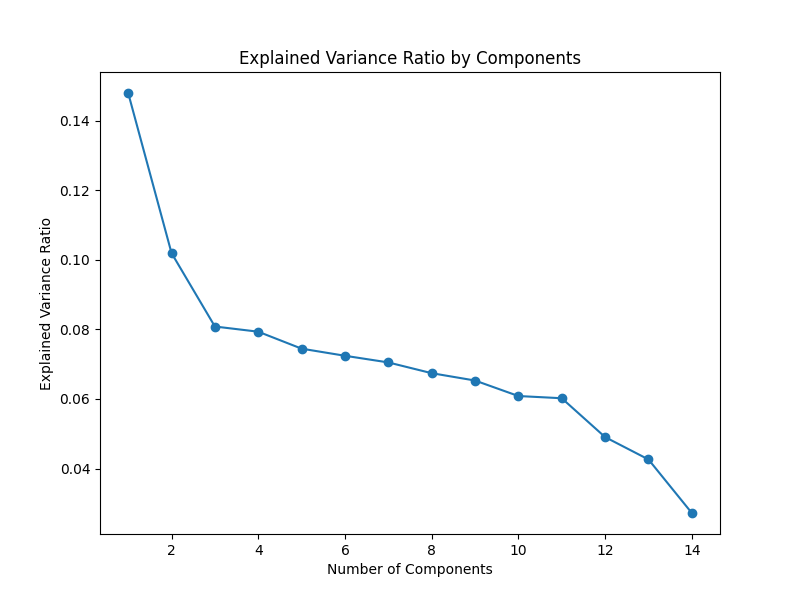
\includegraphics[width=\linewidth]{figure/ACI PCA.png}
    \caption{Explained variance ratio of the components}
    \label{fig:pca_explained_variance}
\end{figure}

\subsection{Model Selection}

After applying PCA, we train multiple classifiers with different algorithms.
In this report, we use the \texttt{PyCaret} library \cite{PyCaret} to build and compare the classifiers.
The classifiers we have tested include:
\begin{itemize}
    \item Light Gradient Boosting Machine
    \item Gradient Boosting Classifier
    \item Random Forest Classifier
    \item Extreme Gradient Boosting
    \item Extra Trees Classifier
    \item K Neighbors Classifier
    \item Ada Boost Classifier
    \item Logistic Regression
    \item SVM - Linear Kernel
    \item Linear Discriminant Analysis
    \item Ridge Classifier
    \item Quadratic Discriminant Analysis
    \item Naive Bayes
    \item Decision Tree Classifier
\end{itemize}

\subsection{Model Evaluation}

We evaluate the performance of the classifiers by comparing their F1 scores, which are calculated using 10-fold cross-validation.

\section{Experiment}

\subsection{Setup}

As mentioned earlier, we preprocess the data by handling missing values, ordinal encoding, and normalization with \texttt{scikit-learn} library \cite{scikit-learn}.
Then, we apply PCA to reduce the dimensionality of the data with \texttt{PyCaret} library.
Finally, we train multiple classifiers with different algorithms and evaluate their performance with 10-fold cross-validation.

\subsection{Results}

\begin{table}[!ht]
    \centering
    \resizebox{\linewidth}{!}{
        \begin{tabular}{llllll}
            \toprule
            \textbf{Model} & \textbf{Accuracy} & \textbf{AUC} & \textbf{Recall} & \textbf{Precision} & \textbf{F1} \\ 
            \midrule
            Light Gradient Boosting Machine & 0.8405 & 0.8928 & 0.5781 & 0.7067 & 0.6357  \\ 
            Gradient Boosting Classifier    & 0.8345 & 0.8818 & 0.519  & 0.7167 & 0.6016  \\ 
            Random Forest Classifier        & 0.8341 & 0.8821 & 0.5362 & 0.7047 & 0.6087  \\ 
            Extreme Gradient Boosting       & 0.8337 & 0.8847 & 0.5763 & 0.6847 & 0.6254  \\ 
            Extra Trees Classifier          & 0.8299 & 0.8765 & 0.5294 & 0.6927 & 0.5998  \\ 
            K Neighbors Classifier          & 0.8247 & 0.8459 & 0.5742 & 0.6556 & 0.612   \\ 
            Ada Boost Classifier            & 0.8243 & 0.8595 & 0.5174 & 0.6776 & 0.5865  \\ 
            Logistic Regression             & 0.8218 & 0.8486 & 0.4391 & 0.7126 & 0.5426  \\ 
            SVM - Linear Kernel             & 0.8125 & 0.8277 & 0.3641 & 0.7191 & 0.4816  \\ 
            Linear Discriminant Analysis    & 0.812  & 0.835  & 0.4011 & 0.6903 & 0.5066  \\ 
            Ridge Classifier                & 0.8058 & 0.835  & 0.3118 & 0.727  & 0.436   \\ 
            Quadratic Discriminant Analysis & 0.8014 & 0.8603 & 0.3121 & 0.6964 & 0.4304  \\ 
            Naive Bayes                     & 0.7764 & 0.7982 & 0.2907 & 0.5705 & 0.3847  \\ 
            Decision Tree Classifier        & 0.7748 & 0.6963 & 0.545  & 0.5316 & 0.538   \\ 
            Dummy Classifier                & 0.7592 & 0.5    & 0      & 0      & 0       \\
            \bottomrule
        \end{tabular}
    }
    \caption{Model evaluation results}
    \label{tab:model_evaluation}
\end{table}

\subsection{Analysis}

As shown in Table \ref{tab:model_evaluation}, the Light Gradient Boosting Machine (LGBM) classifier achieves the best performance with an F1 score of 0.6357.
We can also observe that boosting classifiers obtain 3 of the top 5 F1 scores.
This indicates that boosting is a powerful technique for binary classification problems.

The confusion matrix of the LGBM classifier is shown in Figure \ref{fig:confusion_matrix}.
As we can see, the dataset is imbalanced, with more data points in the 0 class than in the 1 class.
This is why we use the F1 score as the evaluation metric, as it measures the performance of the classifier on imbalanced datasets more effectively than accuracy.

\begin{figure}[!ht]
    \centering
    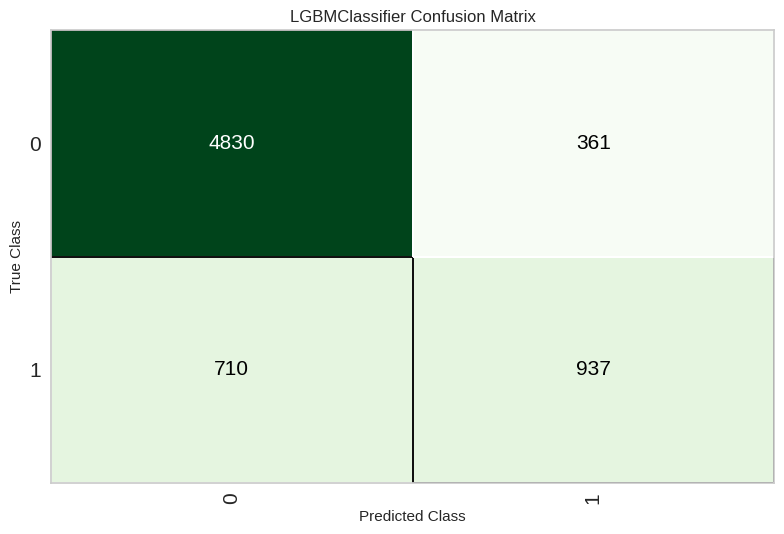
\includegraphics[width=\linewidth]{figure/Confusion Matrix.png}
    \caption{Confusion matrix of the LGBM classifier}
    \label{fig:confusion_matrix}
\end{figure}

Since the light gradient boosting machine is essentially a decision tree-based model, we can visualize the model as tree plot as shown in Figure \ref{fig:lgbm_tree_plot}.
To be noticed, because of the PCA, the features in the tree plot are renamed as ``pca1'', ``pca2'', etc.

\begin{figure}[!ht]
    \centering
    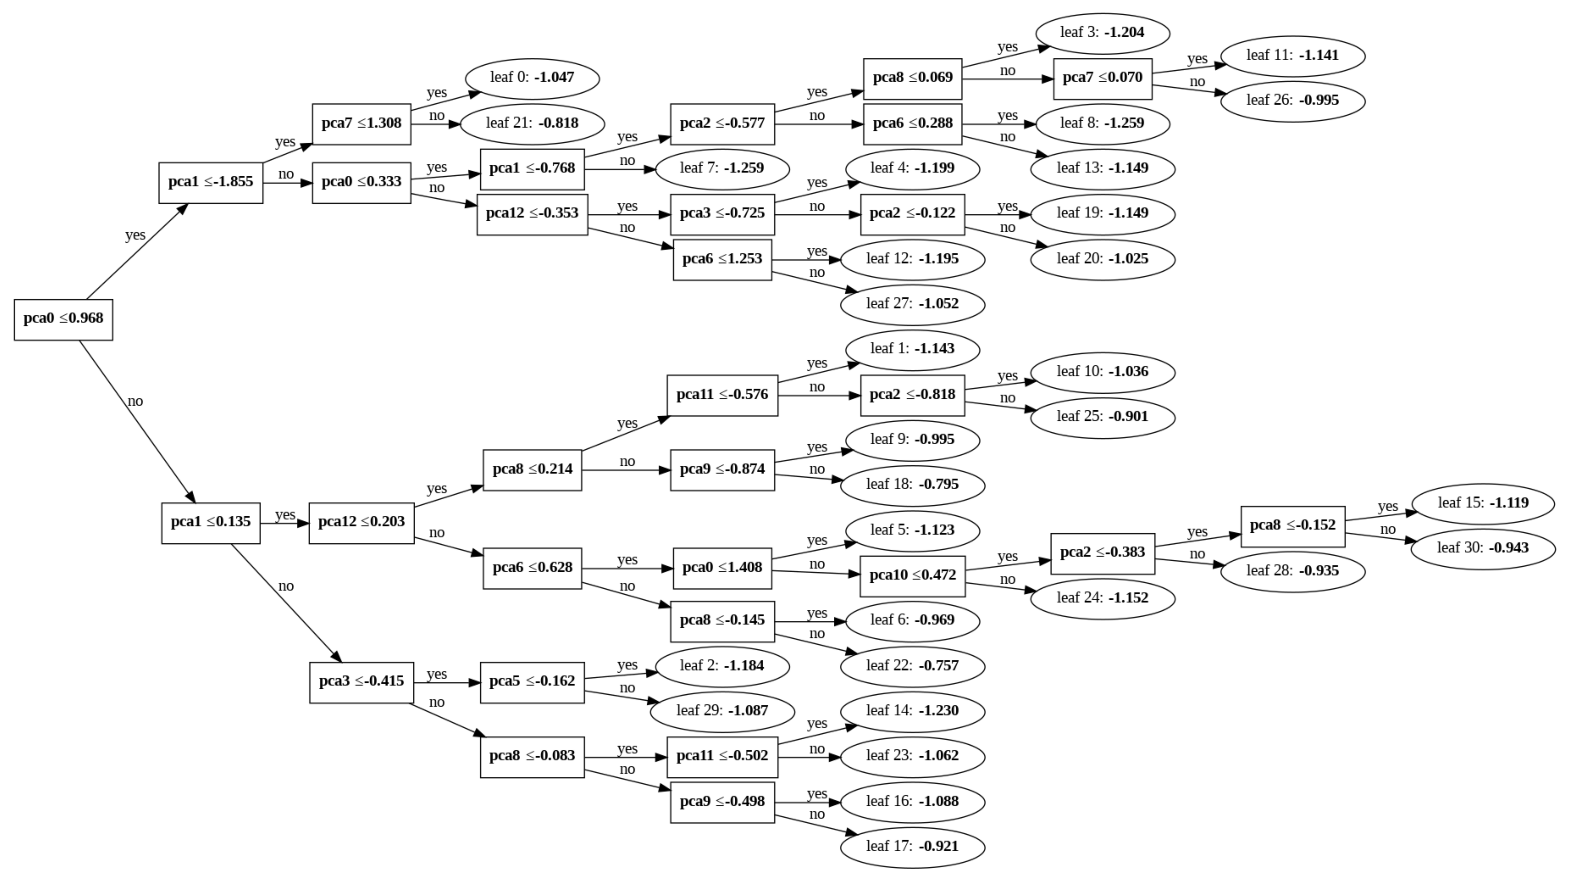
\includegraphics[width=\linewidth]{figure/LGBM Tree Plot.png}
    \caption{Visualization of the LGBM model as a tree plot}
    \label{fig:lgbm_tree_plot}
\end{figure}

\subsection{Discussion}

Although PCA is effective in reducing the dimensionality of the data, it brings challenge to the interpretability of the model.
After PCA, the new features lose their original meanings.
Therefore, though we can still visualize the model as a tree plot, it is difficult to interpret the model in terms of the original features.

\section{Conclusion}

In this report, we present a solution to the Adult Census Income Prediction Problem by applying Principal Component Analysis (PCA) to reduce the dimensionality of the data and then training multiple classifiers with different algorithms.
We evaluate the performance of these classifiers by comparing their F1 scores.
Our results show that the Light Gradient Boosting Machine (LGBM) classifier achieves the best performance with an F1 score of 0.6357.

\printbibliography

\end{document}
